\paragraph{Sơ đồ tuần tự luồng quản lý engine giọng nói}

Luồng nghiệp vụ này mô tả
quy trình quản trị viên
(Admin)
tạo mới hoặc cập nhật Engine giọng nói trong dịch vụ nhân vật.

\begin{figure}[H]
\centering
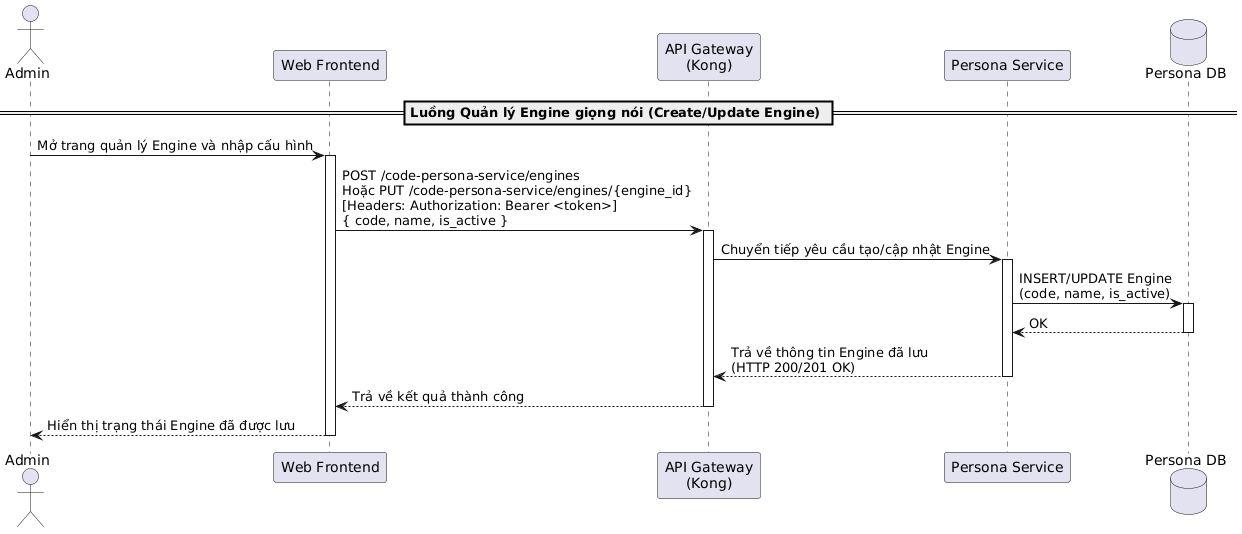
\includegraphics[width=0.95\textwidth]{contents/Sequence/UML-Sequence-AdminManageVoiceEngine.png}
\caption{Sơ đồ tuần tự luồng quản lý engine giọng nói}
\end{figure}

\begin{table}[H]
\centering
\renewcommand{\arraystretch}{1.3}

\begin{tabular}{|l|l|p{5cm}|}
\hline
\textbf{Thành phần} & \textbf{Phân loại} & \textbf{Vai trò trong hệ thống} \\ \hline
Admin & Actor & Quản trị viên
cấu hình mã Engine, tên hiển thị và trạng thái hoạt động. \\ \hline
Web Frontend & Component & Giao diện web Next.js. \\ \hline
API Gateway (Kong) & Component & Cổng API chuyển tiếp các yêu cầu API. \\ \hline
Persona Service & Microservice & Xử lý nghiệp vụ tạo/cập nhật Engine. \\ \hline
Persona Database & Database & Lưu trữ thông tin Engine gồm \texttt{code}, \texttt{name} và \texttt{is\_active}. \\ \hline
\end{tabular}
\caption{Các thành phần tham gia luồng quản lý engine giọng nói}
\end{table}

\subparagraph{Mô tả tổng quan}

\begin{itemize}

\item \textbf{Nhập cấu hình:}
Quản trị viên
nhập thông tin cấu hình của công cụ chuyển đổi giọng nói trên giao diện quản trị.

\item \textbf{Gửi yêu cầu lưu:}
Giao diện gửi yêu cầu tạo mới hoặc cập nhật cấu hình công cụ giọng nói qua cổng API.

\item \textbf{Lưu cấu hình:}
Dịch vụ nhân vật thực hiện lưu trữ hoặc cập nhật thông tin của công cụ giọng nói vào CSDL nhân vật.

\item \textbf{Hoàn tất:}
Hệ thống phản hồi kết quả lưu cấu hình thành công về giao diện hiển thị cho quản trị viên.
\end{itemize}
